\documentclass[12pt]{article}

% Packages for enhanced typesetting and functionality
\usepackage{amsmath, amssymb, amsthm}      % Math symbols and environments
\usepackage{graphicx}                      % For including images
\usepackage{fancyhdr}                      % For header and footer customisation
\usepackage{geometry}                      % For margin customisation
\usepackage[colorlinks=true, linkcolor=blue, urlcolor=blue, citecolor=blue]{hyperref} % Clickable links
\usepackage{xcolor}                        % For coloured text
\usepackage{tikz}                          % For drawing diagrams and flowcharts
\usetikzlibrary{shapes.geometric, arrows.meta, positioning, calc, backgrounds}  % TikZ libraries
\usepackage{algorithm}                     % For algorithms
\usepackage[noend]{algpseudocode}          % For algorithm pseudocode

% Page layout settings
\geometry{margin=1in}
\setlength{\parindent}{0pt}
\setlength{\parskip}{1ex}

% Header and footer
\pagestyle{fancy}
\fancyhf{}
\setlength{\headheight}{15pt}
\fancyhead[L]{Solving Air Crew Scheduling Problems}
\fancyhead[R]{Max Hart}
\fancyfoot[C]{\thepage}

% TikZ styles for flowcharts
\tikzset{
  flowblock/.style={
    rectangle, draw, rounded corners, fill=blue!20, 
    text width=10em, align=center, minimum height=3em, font=\small
  },
  flowdecision/.style={
    diamond, draw, fill=green!20, text width=6em, align=center, aspect=2, font=\small
  },
  flowarrow/.style={
    thick, ->, >=Stealth
  },
  looparrow/.style={
    thick, ->, >=Stealth, bend right=45
  }
}

\begin{document}

% Title Page
\begin{titlepage}
    \centering
    \vspace*{1cm}
    
    % University logo (adjust image file as needed)
    
\includegraphics[width=0.4\textwidth]{UoB.jpg}\par\vspace{1cm}
    
    {\LARGE\bfseries Solving Air Crew Scheduling Problems\par}
    \vspace{0.5cm}
    {\Large A Simulated Annealing and Genetic Algorithms Approach\par}
    \vspace{0.75cm}
    
    {\large Evolutionary Computation\par}
    \vspace{1.5cm}
    
    {\large\textbf{Author:} Max Hart\par}
    \vspace{0.3cm}
    {\normalsize \href{mailto:mah422@student.bham.ac.uk}{mah422@student.bham.ac.uk}\par}
    \vspace{1.5cm}
    
    {\large\textbf{Supervisors:} Dr Shan He and Dr Per Kristian Lehre\par}
    \vspace{1cm}
    
    {\large \today\par}
    
\end{titlepage}

\tableofcontents
\newpage

\section{Introduction}
Airline crew scheduling stands as one of the most challenging and practically significant optimisation problems in the transportation industry. Typically modelled as a Set Partitioning Problem (SPP), it requires that each flight leg be covered exactly once by a valid crew rotation while satisfying a multitude of operational constraints. Conventional exact methods often prove inadequate due to the sheer combinatorial complexity of real-world instances. This has driven the pursuit of advanced metaheuristic approaches, which promise to deliver high-quality, near-optimal solutions within reasonable computational time.

The present project embraces this challenge by developing and implementing three distinct algorithms from scratch: Simulated Annealing (SA), a Standard Binary Genetic Algorithm (BGA), and an Improved Binary Genetic Algorithm (BGA). The improved variant is particularly notable for its incorporation of problem-specific enhancements, including a pseudo–random initialisation method, a heuristic improvement operator (inspired by the DROP/ADD procedure outlined in~\cite{ChuAndBeasley1998}), and a stochastic ranking mechanism for constraint handling as proposed by Runarsson and Yao~\cite{RunarssonYao2000}. Our overarching ambition is to not only demonstrate the correctness and efficiency of these algorithms on three OR–Library test instances (sppnw41, sppnw42, and sppnw43) over 30 independent runs, but also to perform a detailed comparative analysis of their performance, convergence behaviour, and constraint-handling strategies.

This report is structured to provide a comprehensive overview of our methodology and findings. In Section~2, we describe each algorithm in detail with accompanying pseudocode and flowcharts, thereby offering insight into their operational mechanisms. Section~3 presents the benchmark results, including average performance metrics and standard deviations. Section~4 delivers an in-depth discussion and comparison of the algorithms, focusing on their feasibility, convergence speed, and solution quality. Finally, Section~5 addresses the nuances of constraint handling by comparing the deterministic ranking replacement method with the adaptive stochastic ranking approach. Through this work, we aspire to contribute valuable insights into the application of metaheuristic techniques for solving complex, real-world scheduling problems.

\section{Algorithm Descriptions}
\label{sec:algorithms}
This section provides an overview of the three algorithms. For each algorithm, a brief introduction is provided along with the corresponding pseudocode (on the same page). The detailed flowchart for each algorithm is presented on its own centred page.

\newpage

\subsection{Simulated Annealing (SA)}
Simulated Annealing is a local search technique that iteratively improves a candidate solution by exploring its neighbourhood. It uses a temperature parameter to probabilistically accept inferior solutions, thereby enabling the algorithm to escape local optima. This simple yet effective approach balances exploration and exploitation through gradual cooling.

\subsubsection*{Pseudocode}
\begin{algorithm}[htbp]
\caption{SimulatedAnnealing(\(T\), \(\alpha\), maxIter, penaltyFactor)}
\begin{algorithmic}[1]
  \State \(x \gets \text{RandomSolution}()\)
  \State \(F(x) \gets \text{PenaltyFitness}(x,\,\text{penaltyFactor})\)
  \State \(x_{\text{best}} \gets x,\; F_{\text{best}} \gets F(x)\)
  \For{\(iter = 1\) to maxIter}
    \State \(x' \gets \text{FlipOneBit}(x)\)
    \State \(F(x') \gets \text{PenaltyFitness}(x',\,\text{penaltyFactor})\)
    \If{\(F(x') < F(x)\)}
      \State \(x \gets x'\)
    \Else
      \State \(\Delta \gets F(x') - F(x)\)
      \If{\(\text{rand}() < e^{-\Delta/T}\)}
        \State \(x \gets x'\)
      \EndIf
    \EndIf
    \If{\(F(x) < F_{\text{best}}\)}
      \State \(x_{\text{best}} \gets x,\; F_{\text{best}} \gets F(x)\)
    \EndIf
    \State \(T \gets \alpha \, T\)
  \EndFor
  \State \Return \((x_{\text{best}}, F_{\text{best}})\)
\end{algorithmic}
\end{algorithm}

\newpage

\subsubsection*{Flowchart}

\begin{figure}[htbp]
\centering
\resizebox{0.9\textwidth}{!}{
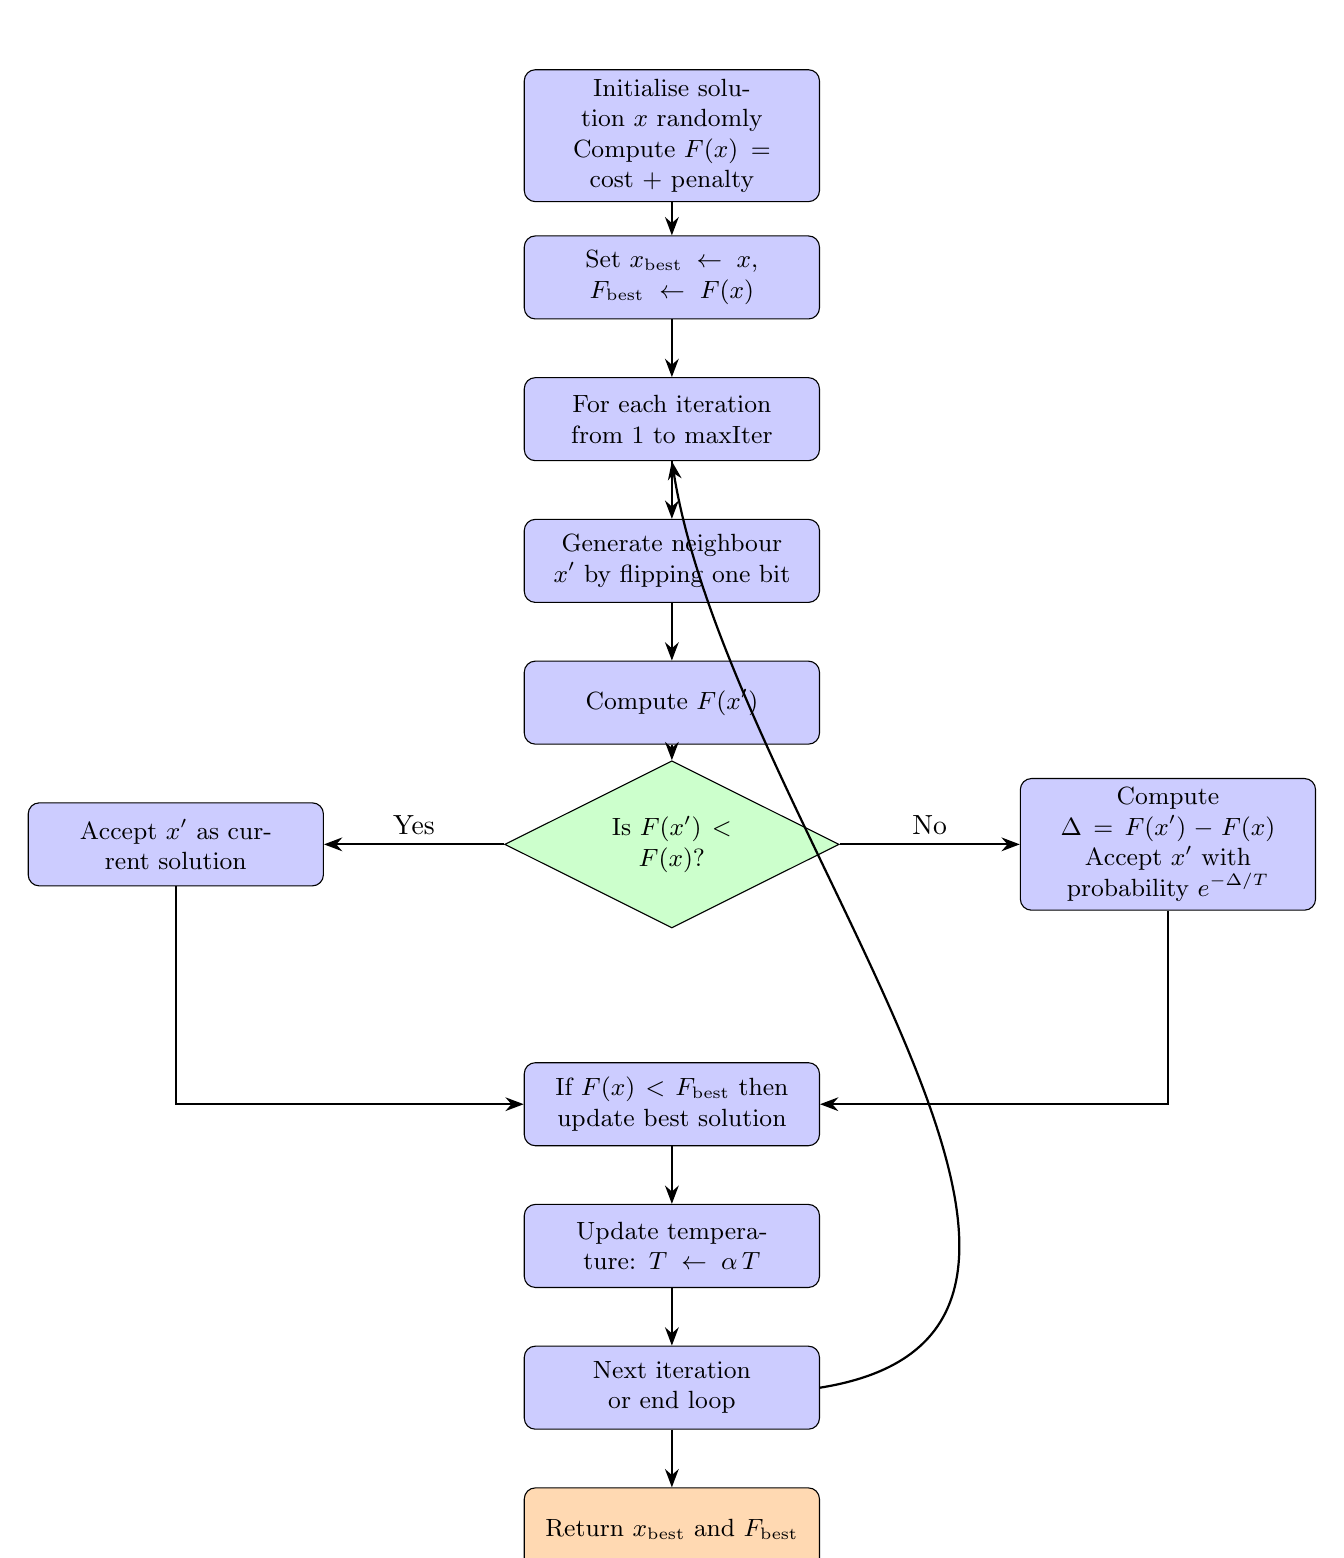
\begin{tikzpicture}[node distance=1.8cm]
  \node[flowblock] (start) {Initialise solution \(x\) randomly\\ Compute \(F(x)=\) cost + penalty};
  \node[flowblock, below of=start] (setbest) {Set \(x_{\text{best}} \gets x\), \(F_{\text{best}} \gets F(x)\)};
  \node[flowblock, below of=setbest] (loop) {For each iteration from 1 to maxIter};
  \node[flowblock, below of=loop] (neighbor) {Generate neighbour \(x'\) by flipping one bit};
  \node[flowblock, below of=neighbor] (evalNeigh) {Compute \(F(x')\)};
  \node[flowdecision, below of=evalNeigh] (better) {Is \(F(x') < F(x)\)?};
  \node[flowblock, left of=better, xshift=-4.5cm] (acceptYes) {Accept \(x'\) as current solution};
  \node[flowblock, right of=better, xshift=4.5cm] (prob) {Compute \(\Delta=F(x')-F(x)\)\\ Accept \(x'\) with probability \(e^{-\Delta/T}\)};
  \node[flowblock, below of=better, yshift=-1.5cm] (updateBest) {If \(F(x) < F_{\text{best}}\) then update best solution};
  \node[flowblock, below of=updateBest] (cool) {Update temperature: \(T \gets \alpha \, T\)};
  \node[flowblock, below of=cool] (next) {Next iteration or end loop};
  \node[flowblock, below of=next, fill=orange!30] (end) {Return \(x_{\text{best}}\) and \(F_{\text{best}}\)};
  
  \draw[flowarrow] (start) -- (setbest);
  \draw[flowarrow] (setbest) -- (loop);
  \draw[flowarrow] (loop) -- (neighbor);
  \draw[flowarrow] (neighbor) -- (evalNeigh);
  \draw[flowarrow] (evalNeigh) -- (better);
  \draw[flowarrow] (better) -- node[above,align=center]{Yes} (acceptYes);
  \draw[flowarrow] (better) -- node[above,align=center]{No} (prob);
  \draw[flowarrow] (acceptYes) |- (updateBest);
  \draw[flowarrow] (prob) |- (updateBest);
  \draw[flowarrow] (updateBest) -- (cool);
  \draw[flowarrow] (cool) -- (next);
  \draw[looparrow] (next) to [out=-90, in=180] (loop);
  \draw[flowarrow] (next) -- (end);
\end{tikzpicture}
}
\caption{Flowchart for Simulated Annealing.}
\label{fig:sa_flowchart}
\end{figure}

\newpage

\subsection{Standard Binary Genetic Algorithm (BGA)}
The Standard Binary Genetic Algorithm is a population-based technique that evolves a set of candidate solutions using selection, crossover, and mutation operators. It utilises tournament selection to choose parents, applies one-point crossover to combine their genetic material, and uses bit-flip mutation to introduce variability. A penalty function is employed to combine the cost of a solution with constraint violations, ensuring that feasibility is encouraged over generations. This method is well-suited for problems with discrete binary representations and offers robustness through its stochastic operations.

\subsubsection*{Pseudocode}
\begin{algorithm}[htbp]
\caption{StandardBGA(popSize, cxRate, mutRate, maxGens, penaltyFactor)}
\begin{algorithmic}[1]
  \State \(P \gets \text{RandomPopulation}(popSize)\)
  \State \(\text{EvaluateFitness}(P,\,\text{penaltyFactor})\)
  \For{\(g = 1\) to maxGens}
    \State \(Q \gets \emptyset\)
    \While{\(|Q| < \text{popSize}\)}
      \State \(p_1 \gets \text{TournamentSelect}(P)\)
      \State \(p_2 \gets \text{TournamentSelect}(P)\)
      \If{\(\text{rand}() < cxRate\)}
        \State \((c_1, c_2) \gets \text{OnePointCrossover}(p_1, p_2)\)
      \Else
        \State \(c_1 \gets p_1,\; c_2 \gets p_2\)
      \EndIf
      \State \(\text{Mutate}(c_1,\, mutRate)\)
      \State \(\text{Mutate}(c_2,\, mutRate)\)
      \State \(\text{EvaluateFitness}(\{c_1, c_2\},\, \text{penaltyFactor})\)
      \State \(Q \gets Q \cup \{c_1, c_2\}\)
    \EndWhile
    \State \(P \gets Q\)
  \EndFor
  \State \Return \(\text{BestSolution}(P)\)
\end{algorithmic}
\end{algorithm}

\newpage

\subsubsection*{Flowchart}
\begin{figure}[htbp]
\centering
\resizebox{0.50\textwidth}{!}{
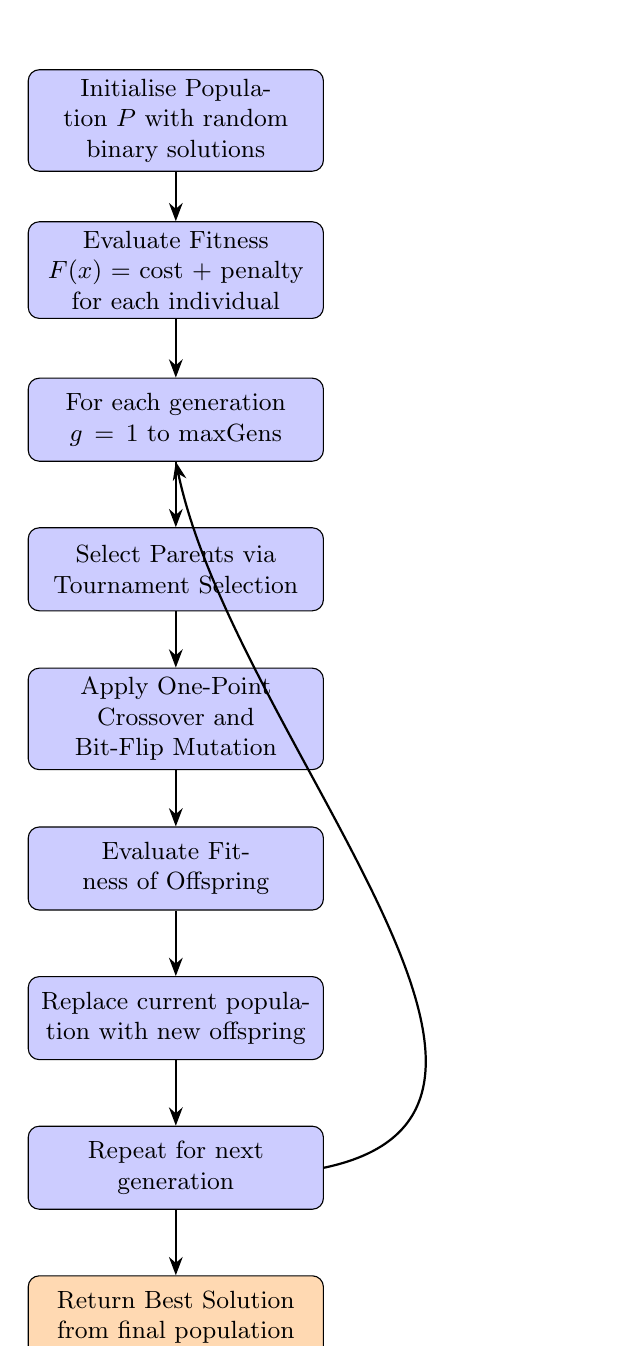
\begin{tikzpicture}[node distance=1.9cm]
  \node[flowblock] (init) {Initialise Population \(P\) with random binary solutions};
  \node[flowblock, below of=init] (eval) {Evaluate Fitness \(F(x)=\) cost + penalty for each individual};
  \node[flowblock, below of=eval] (genLoop) {For each generation \(g=1\) to maxGens};
  \node[flowblock, below of=genLoop] (select) {Select Parents via Tournament Selection};
  \node[flowblock, below of=select] (variation) {Apply One-Point Crossover and Bit-Flip Mutation};
  \node[flowblock, below of=variation] (evalOff) {Evaluate Fitness of Offspring};
  \node[flowblock, below of=evalOff] (replace) {Replace current population with new offspring};
  \node[flowblock, below of=replace] (loopBack) {Repeat for next generation};
  \node[flowblock, below of=loopBack, fill=orange!30] (end) {Return Best Solution from final population};
  
  \draw[flowarrow] (init) -- (eval);
  \draw[flowarrow] (eval) -- (genLoop);
  \draw[flowarrow] (genLoop) -- (select);
  \draw[flowarrow] (select) -- (variation);
  \draw[flowarrow] (variation) -- (evalOff);
  \draw[flowarrow] (evalOff) -- (replace);
  \draw[flowarrow] (replace) -- (loopBack);
  \draw[looparrow] (loopBack) to [out=-90, in=180] (genLoop);
  \draw[flowarrow] (loopBack) -- (end);
\end{tikzpicture}
}
\caption{Flowchart for Standard Binary Genetic Algorithm.}
\label{fig:bga_flowchart}
\end{figure}

\newpage

\subsection{Improved Binary Genetic Algorithm (BGA)}
The Improved Binary Genetic Algorithm extends the standard BGA by integrating several problem-specific enhancements. It begins with a pseudo–random initialisation that aims to reduce over–coverage in the initial population. The algorithm then incorporates a stochastic ranking procedure that probabilistically balances cost and constraint violation, allowing for a more flexible handling of infeasible solutions. Adaptive mutation is employed to reintroduce promising genetic material, and a DROP/ADD heuristic improvement operator repairs infeasible solutions. These enhancements, inspired by Chu \& Beasley~\cite{ChuAndBeasley1998} and Runarsson \& Yao~\cite{RunarssonYao2000}, make the Improved BGA particularly robust for the SPP. Overall, this algorithm offers a more sophisticated search mechanism by blending global search operators with domain-specific repairs.

\subsubsection*{Pseudocode}
\begin{algorithm}[htbp]
\caption{ImprovedBGA(popSize, maxGens, \(p_{\mathrm{stoch}}\), ...)}
\begin{algorithmic}[1]
  \State \(P \gets \text{PseudoRandomInit}(popSize)\)
  \State \(\text{EvaluateCostUnfitness}(P)\)
  \For{\(g = 1\) to maxGens}
    \State \(\text{StochasticRankSort}(P, p_{\mathrm{stoch}})\)
    \State \(O \gets \emptyset\)
    \While{\(|O| < popSize\)}
      \State \((p_1, p_2) \gets \text{SelectParents}(P)\)
      \State \((c_1, c_2) \gets \text{UniformCrossover}(p_1, p_2)\)
      \State \(\text{AdaptiveMutation}(c_1, P)\)
      \State \(\text{AdaptiveMutation}(c_2, P)\)
      \State \(\text{HeuristicImprove}(c_1)\)
      \State \(\text{HeuristicImprove}(c_2)\)
      \State \(\text{EvaluateCostUnfitness}(\{c_1, c_2\})\)
      \State \(O \gets O \cup \{c_1, c_2\}\)
    \EndWhile
    \State \(C \gets P \cup O\)
    \State \(\text{StochasticRankSort}(C, p_{\mathrm{stoch}})\)
    \State \(P \gets \text{Top}(C, popSize)\)
  \EndFor
  \State \Return \(\text{BestFeasible}(P)\)
\end{algorithmic}
\end{algorithm}

\newpage

\subsubsection*{Flowchart}
\begin{figure}[htbp]
\centering
\resizebox{0.45\textwidth}{!}{
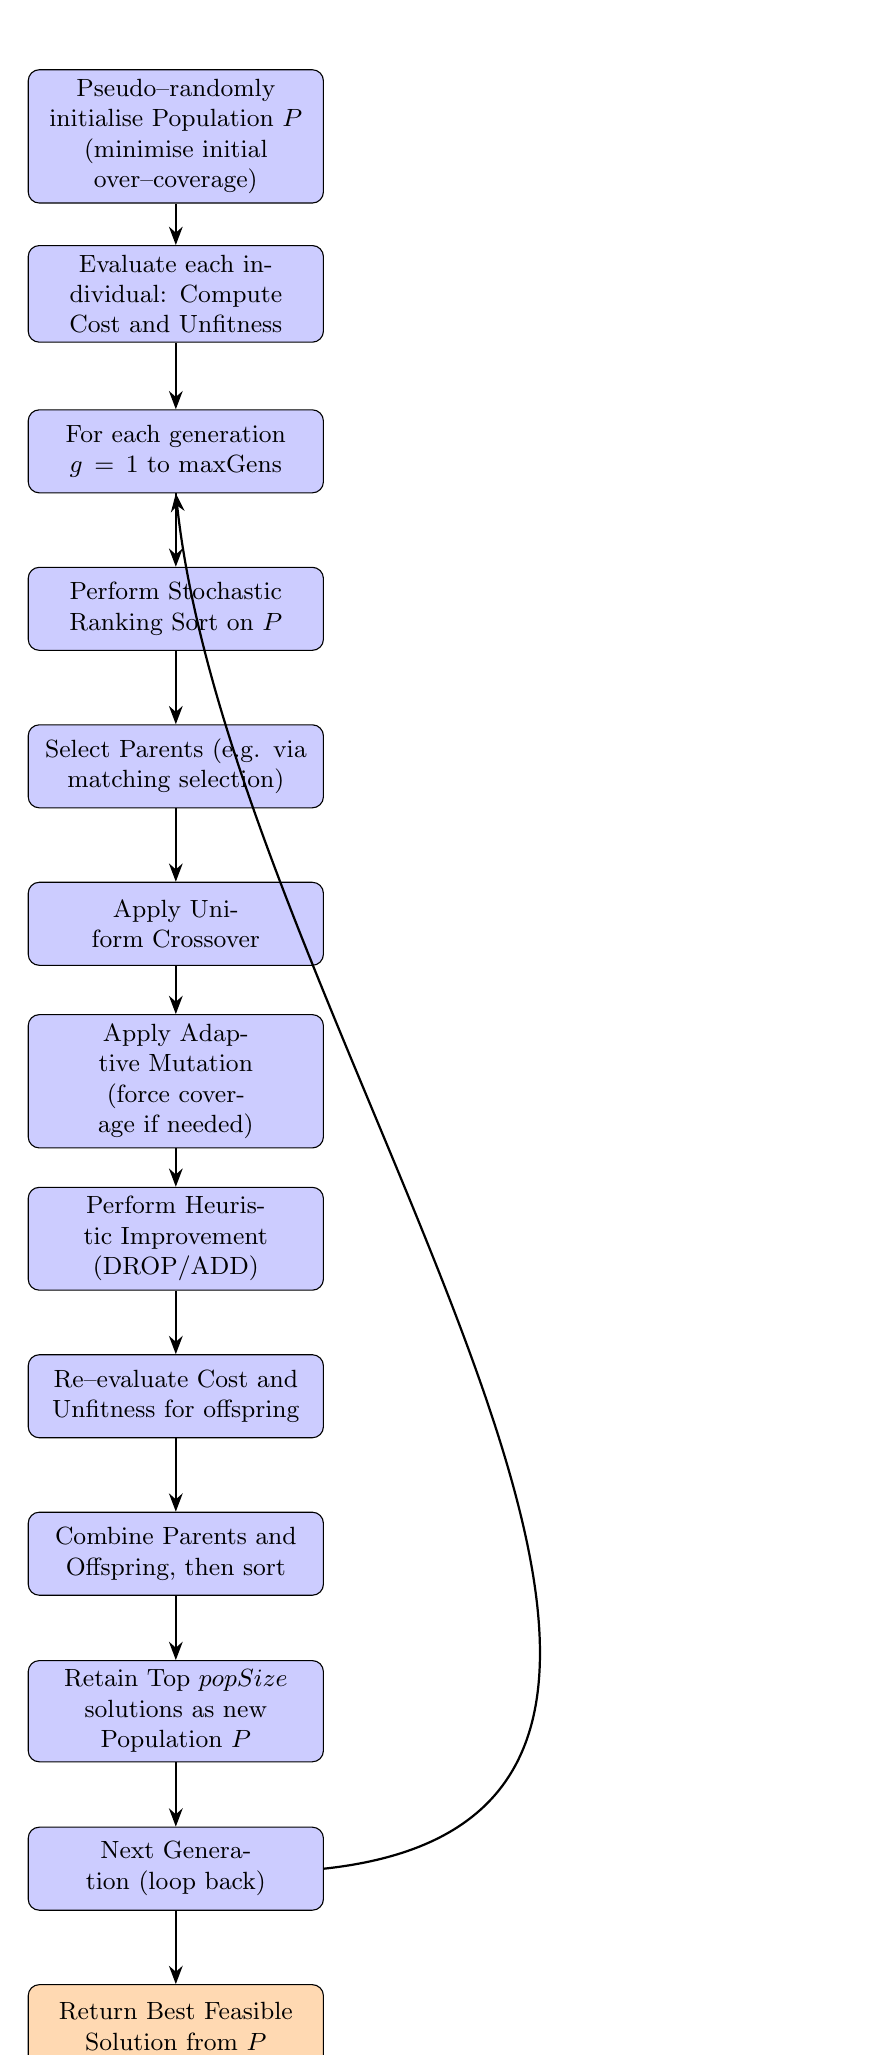
\begin{tikzpicture}[node distance=2cm]
  \node[flowblock] (init) {Pseudo–randomly initialise Population \(P\)\\ (minimise initial over–coverage)};
  \node[flowblock, below of=init] (eval) {Evaluate each individual: Compute Cost and Unfitness};
  \node[flowblock, below of=eval] (genLoop) {For each generation \(g=1\) to maxGens};
  \node[flowblock, below of=genLoop] (stoch) {Perform Stochastic Ranking Sort on \(P\)};
  \node[flowblock, below of=stoch] (select) {Select Parents (e.g. via matching selection)};
  \node[flowblock, below of=select] (crossover) {Apply Uniform Crossover};
  \node[flowblock, below of=crossover] (adaptive) {Apply Adaptive Mutation\\ (force coverage if needed)};
  \node[flowblock, below of=adaptive] (improve) {Perform Heuristic Improvement (DROP/ADD)};
  \node[flowblock, below of=improve] (reeval) {Re–evaluate Cost and Unfitness for offspring};
  \node[flowblock, below of=reeval] (combine) {Combine Parents and Offspring, then sort};
  \node[flowblock, below of=combine] (retain) {Retain Top \(popSize\) solutions as new Population \(P\)};
  \node[flowblock, below of=retain] (loopBack) {Next Generation (loop back)};
  \node[flowblock, below of=loopBack, fill=orange!30] (end) {Return Best Feasible Solution from \(P\)};
  
  \draw[flowarrow] (init) -- (eval);
  \draw[flowarrow] (eval) -- (genLoop);
  \draw[flowarrow] (genLoop) -- (stoch);
  \draw[flowarrow] (stoch) -- (select);
  \draw[flowarrow] (select) -- (crossover);
  \draw[flowarrow] (crossover) -- (adaptive);
  \draw[flowarrow] (adaptive) -- (improve);
  \draw[flowarrow] (improve) -- (reeval);
  \draw[flowarrow] (reeval) -- (combine);
  \draw[flowarrow] (combine) -- (retain);
  \draw[flowarrow] (retain) -- (loopBack);
  \draw[looparrow] (loopBack) to [out=-90, in=180] (genLoop);
  \draw[flowarrow] (loopBack) -- (end);
\end{tikzpicture}
}
\caption{Flowchart for Improved Binary Genetic Algorithm.}
\label{fig:improved_bga_flowchart}
\end{figure}

\newpage

\section{Benchmark Results}
\label{sec:results}

\section{Discussion and Comparison}
\label{sec:discussion}


\section{Ranking Replacement vs. Stochastic Ranking}
\label{sec:ranking}
Handling constraints is critical in the SPP. Two notable methods are:

\subsection*{Ranking Replacement (Chu \& Beasley, 1998)}
This method partitions the population into four subgroups based on fitness (cost) and unfitness (constraint violation). A new solution replaces a member from the first non-empty subgroup (starting with those worse in both criteria). This deterministic approach systematically reduces infeasibility while improving cost.

\subsection*{Stochastic Ranking (Runarsson \& Yao, 2000)}
Stochastic ranking avoids the arduous tuning of penalty coefficients by introducing randomness during comparisons. With a given probability, adjacent individuals are compared solely on cost; otherwise, the comparison is based on unfitness. This probabilistic strategy allows the exploration of infeasible regions as bridges to high-quality, feasible solutions.

\subsection*{Comparison}
While both methods strive to balance solution quality and constraint satisfaction, ranking replacement enforces a strict hierarchical structure, whereas stochastic ranking flexibly blends objective and constraint criteria through randomness. The improved BGA leverages stochastic ranking to adapt to the evolving population without requiring labour-intensive penalty tuning.

\section{Conclusion}
This report has presented three advanced algorithms for solving airline crew scheduling problems: Simulated Annealing, a Standard Binary Genetic Algorithm, and an Improved Binary Genetic Algorithm incorporating problem-specific enhancements. Detailed, moderately sized flowcharts and refined pseudocode have been provided to elucidate each method's internal workings. Benchmark results and an in-depth discussion will be appended once experiments are complete. Furthermore, a comparative discussion on constraint-handling—contrasting ranking replacement and stochastic ranking—has been included, underscoring the adaptive advantages of the latter.

\newpage

\begin{thebibliography}{9}
\bibitem{ChuAndBeasley1998}
  P.~C. Chu and J.~E. Beasley, 
  \emph{Constraint Handling in Genetic Algorithms: The Set Partitioning Problem},
  Journal of Heuristics, 11:323--357, 1998.

\bibitem{RunarssonYao2000}
  T.~P. Runarsson and X. Yao, 
  \emph{Stochastic Ranking for Constrained Evolutionary Optimisation},
  IEEE Transactions on Evolutionary Computation, 4(3):284--294, 2000.
\end{thebibliography}

\end{document}